\section{Thermoelastic stress analysis in composite materials (3~D)}
\subsection{Definition}
If there are two materials with different thermal expansions, the volume changes of the materials will be uncommon. The material with the higher thermal expansion expands more than the material with the low thermal expansion. If deformations at the outer boundaries are prevented, different states of stress will occur in these two materials. But the stresses perpendicular to the parting plane must be equal. The values of the stresses as a result of temperature changes can also easily be calculated by the Hooke's linear elastic model. The aim of this simulation is to specify the stresses at several areas in the solid. Figure \ref{fig64} shows a sketch of the calculation area. The model parameters are given in Table \ref{tab62}.

\begin{figure}[htbp]
\centering
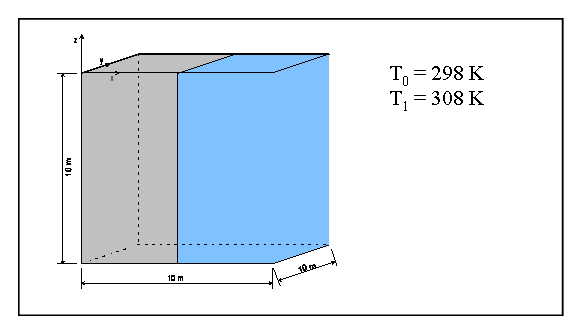
\includegraphics[width=0.6\textwidth]{PART_III/TM/figures/fig64}
\caption{Calculation area with two different materials}
\label{fig64}
\end{figure}

\begin{table}[htbp]
\centering
\caption{Model parameters}
\label{tab62}
\begin{tabular}{llrr}
\toprule
Symbol & Parameter & Value & Unit \\
\midrule
$T_0$  & Initial temperature (before heating) & 298 & $K$ \\
$T_1$  & Temperature after heating & 308 & $K$ \\
$\rho$  & Density of the solid &  2200 & $kg\cdot m^{-3}$  \\			
$E$ & Young's modulus of the solid & 25 & $GPa$ \\
$\nu$ & Poisson ratio & 0.27 & $-$ \\
$\alpha_1$ & Linear thermal expansion of material 1 & 6.0$\cdot$10$^{-6}$ & $K^{-1}$ \\
$\alpha_2$ & Linear thermal expansion of material 2 & 1.2$\cdot$10$^{-5}$ & $K^{-1}$ \\
$c$      & Specific heat capacity & 1.0 & $J\cdot kg^{-1}\cdot K^{-1}$ \\
$\lambda$ & Thermal conductivity & 1.0 & $W\cdot m^{-1}\cdot K^{-1}$ \\
\bottomrule
\end{tabular}
\end{table}

%\newpage

\subsection{Solution}
\subsubsection{Analytical solution}
The equations of the mechanical behaviour base on the Hooke's law for linear elastic materials (see equations \eqref{eq61} to \eqref{eq63}). The analytical solution can be derived from these time independent equations with the assumptions of suppressed deformations in $y$- and $z$-direction and an isotropic thermal expansion:
\begin{displaymath}
\varepsilon_x\,=\,\varepsilon_z\,\equiv\,0
\end{displaymath}
Additionally the stresses in x-direction (perpendicular to the parting plane between the two materials) must be equal:
\begin{displaymath}
\sigma_{x1}\,=\,\sigma_{x2}
\end{displaymath}
where indices denote different materials. 
Further the expansion of the one material leads to a compression of the other material with the same value in x-direction:
\begin{displaymath}
\varepsilon_{x1}\,=\,-\varepsilon_{x2}
\end{displaymath}
With these limiting conditions the analytical solutions are:
\begin{eqnarray}
\varepsilon_{x1} & = &
\frac{\Delta T}{2}\cdot\left(\alpha_1-\alpha_2\right)\cdot
\left(\frac{1+\nu}{1-\nu}\right)
\label{eq65} \\[1.5ex]
\varepsilon_{x2} & = & -\varepsilon_{x1}\,=\,
-\frac{\Delta T}{2}\cdot\left(\alpha_1-\alpha_2\right)\cdot
\left(\frac{1+\nu}{1-\nu}\right)
\label{eq66} \\[1.5ex]
\sigma_{x1} & = & \sigma_{x2}\,=\, E\cdot
\frac{\varepsilon_{x2}\cdot\left(1-\nu\right)-\alpha_2\cdot\Delta T\cdot\left(1+\nu\right)}{1-\nu-2\nu^2}
\label{eq67} \\[1.5ex]
\sigma_{y1} & = & \sigma_{z1}\,=\,
\frac{\nu\cdot\sigma_{x1}-\alpha_1\cdot\Delta T\cdot E}{1-\nu}
\label{eq68} \\[1.5ex]
\sigma_{y2} & = & \sigma_{z2}\,=\,
\frac{\nu\cdot\sigma_{x2}-\alpha_2\cdot\Delta T\cdot E}{1-\nu}
\label{eq69}
\end{eqnarray}
%{\small
%indices:
%
%\begin{tabbing}
%\=xxxx  \=xxxxxxxxxxxxxxxxxxxxxxx \kill
%\> 1 -- \> material 1 \\[1.0ex]
%\> 2 -- \> material 2
%\end{tabbing}
%}

Equations \eqref{eq65} to \eqref{eq69} provide the strains and stresses after heating the body of two materials. The state of stress is anisotropic.


\subsubsection{Numerical solution}
The calculation was done with a 3~D model. The $xy$-plane is the horizontal plane. The height of the body is in $z$-direction. The dimensions of this 3~D model are 10~m in all directions. The model includes 1000 hexahedral elements and 1331 nodes. Deformations perpendicular to the outer surfaces are suppressed. 
%Deformations in $x$- and $z$-direction are suppressed. 
The initial temperature in the whole area is 298~K. At the top and at the bottom of the model thermal boundary conditions are set with a temperature of 308~K. Thereby the heating of the body about 10~K is simulated. The used parameters of the solids represent the material behaviour of concrete. The calculation is divided in 1000 time steps with a constant time step length of 0.5 seconds. A sketch of the calculation model is shown in Figure \ref{fig65}.

\begin{figure}[htbp]
\centering
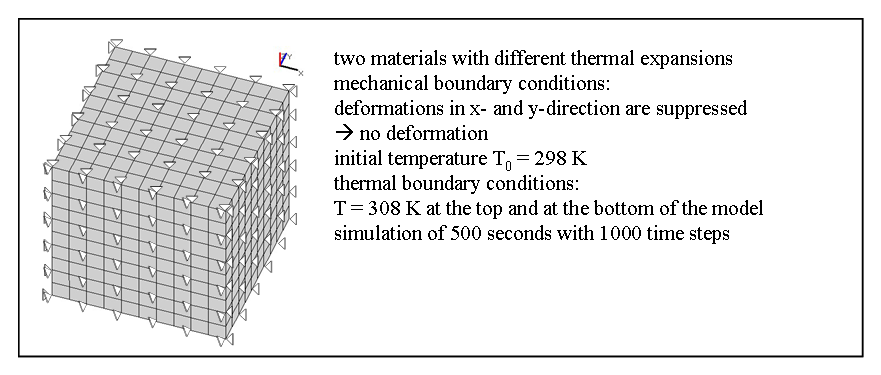
\includegraphics[width=0.6\textwidth]{PART_III/TM/figures/fig65}
\caption{Mesh for TM coupling 3D model with 2 materials}
\label{fig65}
\end{figure}



\subsection{Results}

With the analytical solution in equations \eqref{eq65} to \eqref{eq69} and the used parameters the values of the strains in $x$-direction at the parting plane amount
\begin{eqnarray*}
\varepsilon_{x1} & = & -5.219178\cdot 10^{-5} \\[1.5ex]
\varepsilon_{x2} & = & \phantom{-}5.219178\cdot 10^{-5}
\end{eqnarray*}
The values of the stresses are
\begin{eqnarray*}
\sigma_{x1} & = & \sigma_{x2}\,=\,-4891304.34\,\mathrm{Pa}
                             \,=\,-4.8913\,\mathrm{MPa} \\[1.5ex]
\sigma_{y1} & = & \sigma_{z1}\,=\,-3863907.08\,\mathrm{Pa}
                             \,=\,-3.8639\,\mathrm{MPa} \\[1.5ex]
\sigma_{y2} & = & \sigma_{z2}\,=\,-5918701.60\,\mathrm{Pa}
                             \,=\,-5.9187\,\mathrm{MPa}
\end{eqnarray*}
This anisotropic state of stress is reached after the whole body is heated. The temporal stress developments in several nodes calculated with both RockFlow and OGS are presented in Figure \ref{fig66} and Figure \ref{fig67}.
The results of the 3D simulation show an exact agreement with the analytical solutions.

\begin{figure}[!htbp]
\centering
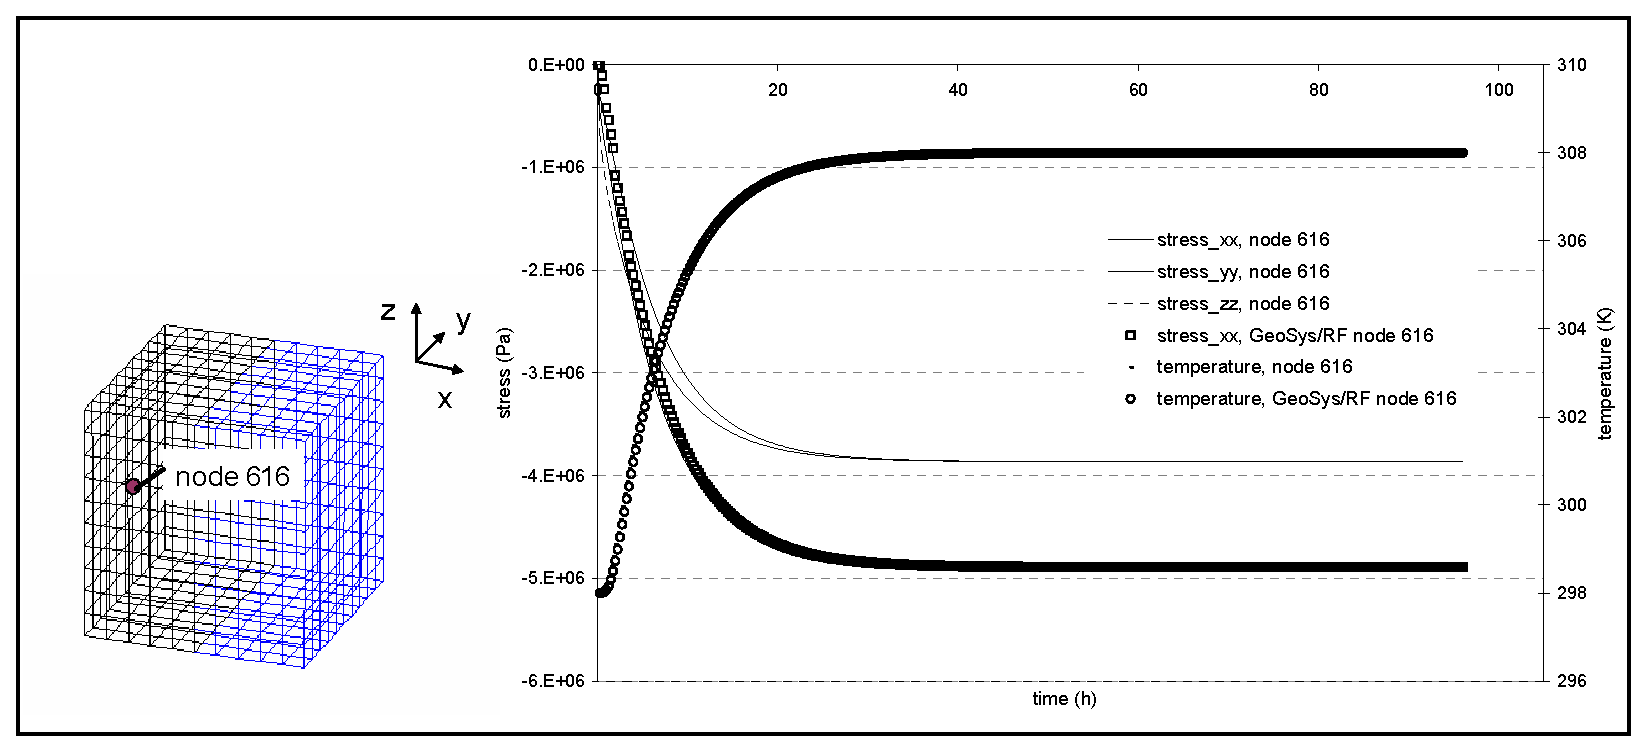
\includegraphics[width=125mm]{PART_III/TM/figures/fig66}
\caption{Temporal stress development in node 616}
\label{fig66}
\end{figure}

\begin{figure}[!htbp]
\centering
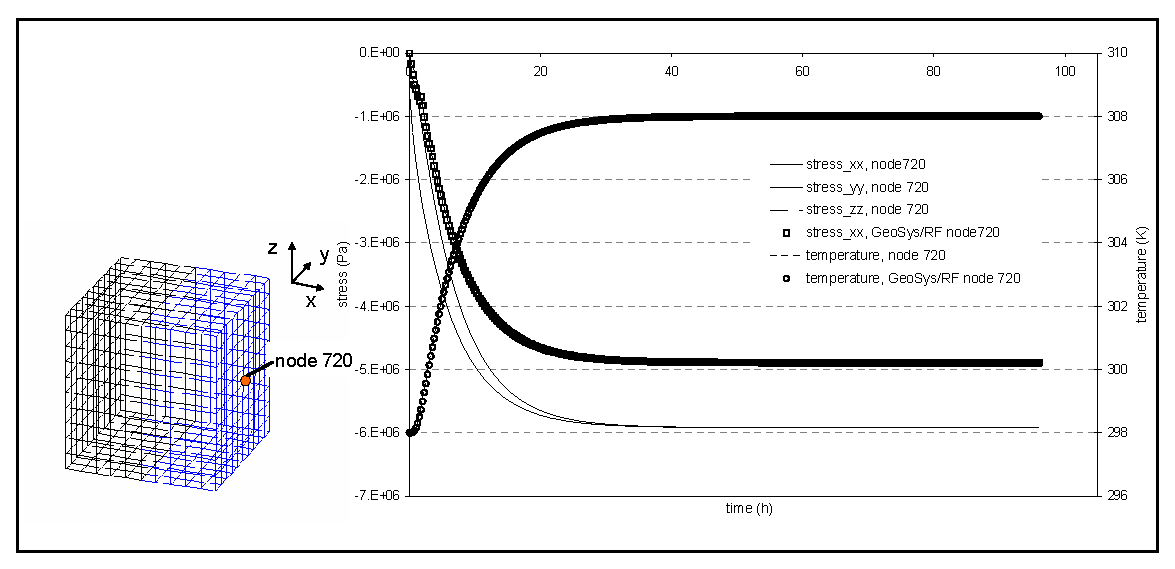
\includegraphics[width=125mm]{PART_III/TM/figures/fig67}
\caption{Temporal stress development in node 720}
\label{fig67}
\end{figure}


